% ============================================================
% ============================================================
% NACA0012 -- DROPLET IMPINGEMENT
% ============================================================
% ============================================================

\section[Impingement]{\textbf{Droplet Impingement}}


% ============================================================
% NACA0012 -- Collection Efficiency Profiles
% ============================================================

\begin{frame}[shrink]{\small NACA0012 -- Collection Efficiency}
\scriptsize

{\centering
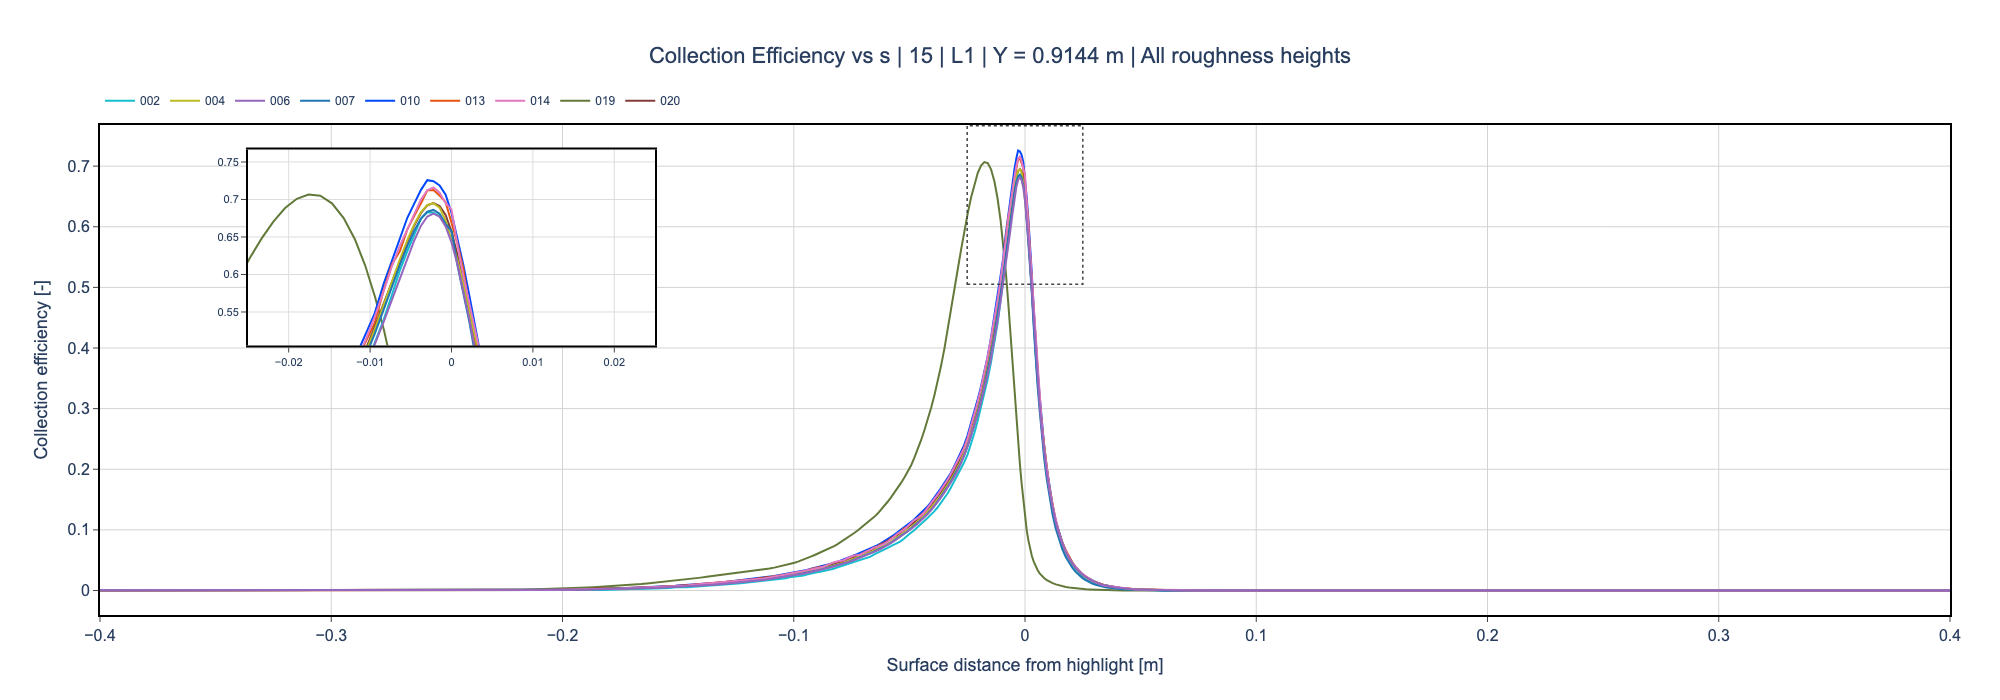
\includegraphics[width=1.0\textwidth]{FIGURES/IMPINGEMENT/tc_naca0012_ae3932_L1_beta_bins15_vs_s_slice_0p9144_all_roughness.png}
\par}

\vspace{0.15cm}

\begin{block}{\scriptsize Assessment}
\begin{itemize}
    \item Most submissions predict a similar collection-efficiency distribution around the leading edge.
    \item Peak collection efficiencies are closely clustered, while differences remain in the detailed profile and impingement extent.
    \item Differences in prescribed surface roughness should be considered when interpreting the remaining code-to-code variability.
\end{itemize}
\end{block}

\end{frame}


% ============================================================
% ============================================================
% NACA0012 -- Collection Efficiency Grid Convergence
% ============================================================
% ============================================================

\begin{frame}{\small NACA0012 -- Collection Efficiency Grid Convergence}
\scriptsize

\begin{columns}[T,onlytextwidth]

\begin{column}{0.50\textwidth}
    \centering
    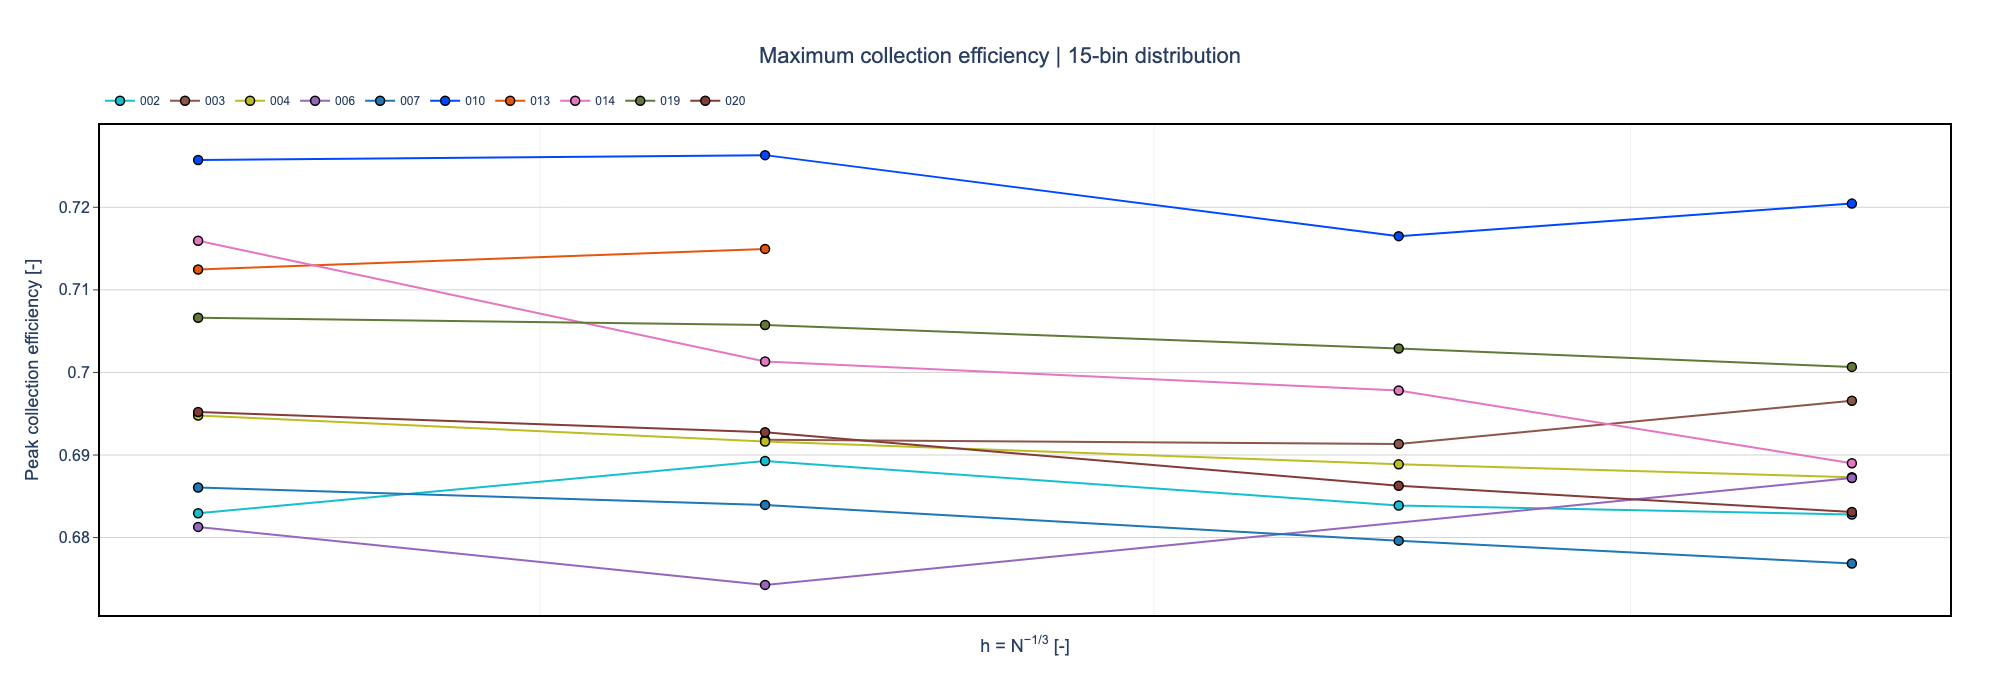
\includegraphics[width=\textwidth]{FIGURES/IMPINGEMENT/tc_naca0012_ae3932_beta_max_bins15.png}
\end{column}

\begin{column}{0.50\textwidth}
    \centering
    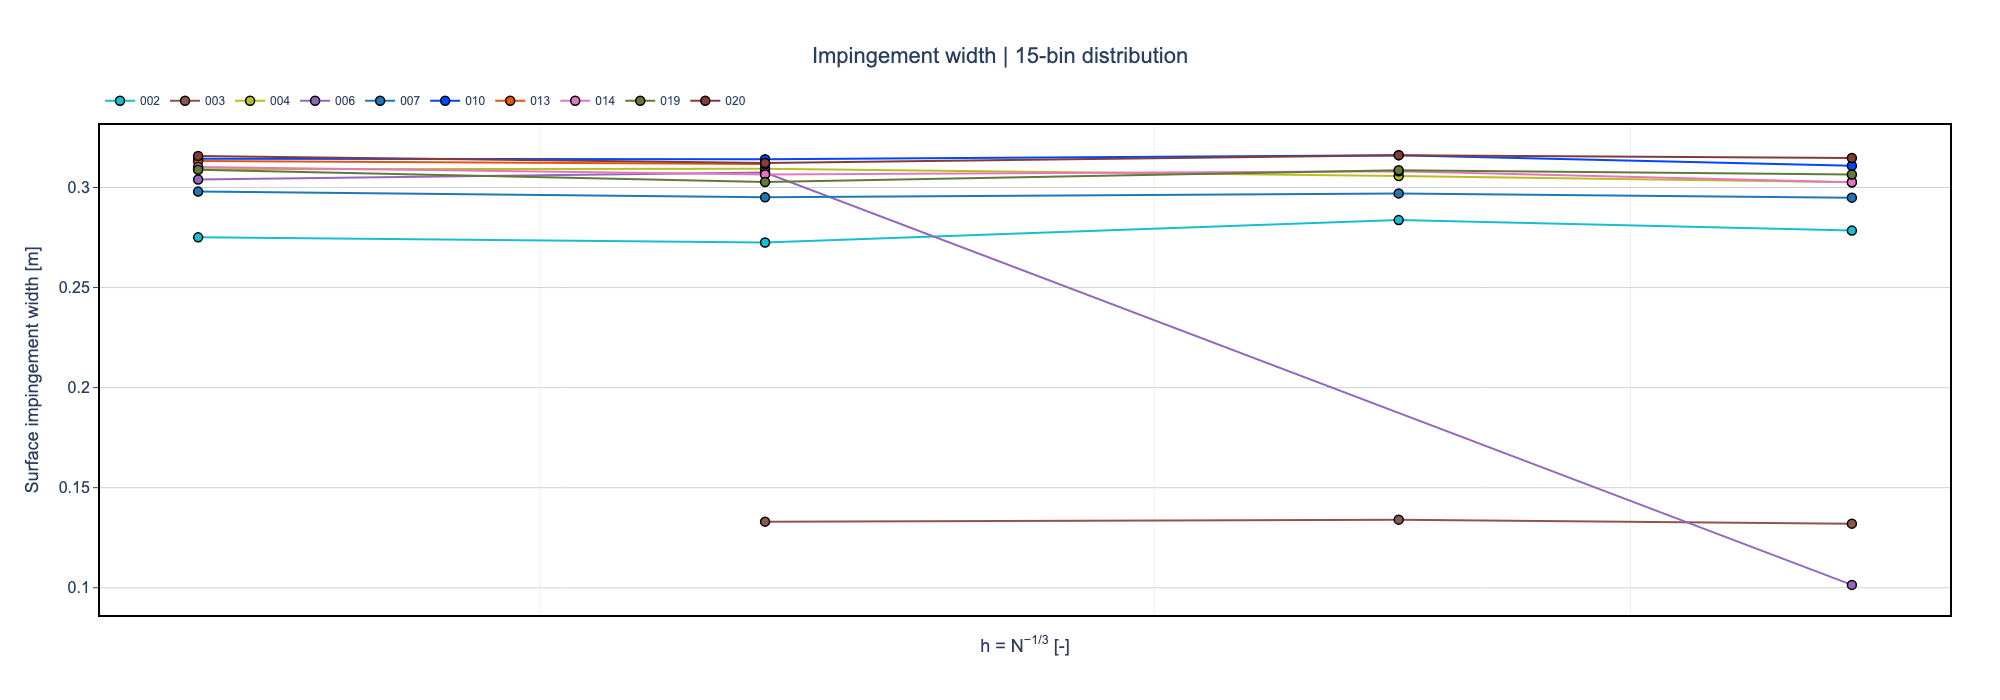
\includegraphics[width=\textwidth]{FIGURES/IMPINGEMENT/tc_naca0012_ae3932_width_bins15.png}
\end{column}

\end{columns}

\vspace{0.15cm}

\begin{block}{\scriptsize Assessment}
\begin{itemize}
    \item At L1, the median peak collection efficiency is $\beta_{\max}=0.695$ with an IQR of $0.0209$ ($3.0\%$).
    \item The L1 median impingement width is $0.309~\mathrm{m}$ with an IQR of $8.93\times10^{-3}~\mathrm{m}$ ($2.9\%$).
    \item Both quantities exhibit limited grid sensitivity for most submissions, indicating comparatively stable local impingement predictions.
\end{itemize}
\end{block}

\end{frame}


% ============================================================
% ============================================================
% NACA0012 -- Water Mass Grid Convergence
% ============================================================
% ============================================================

\begin{frame}{\small NACA0012 -- Water Mass Grid Convergence}
\scriptsize

{\centering
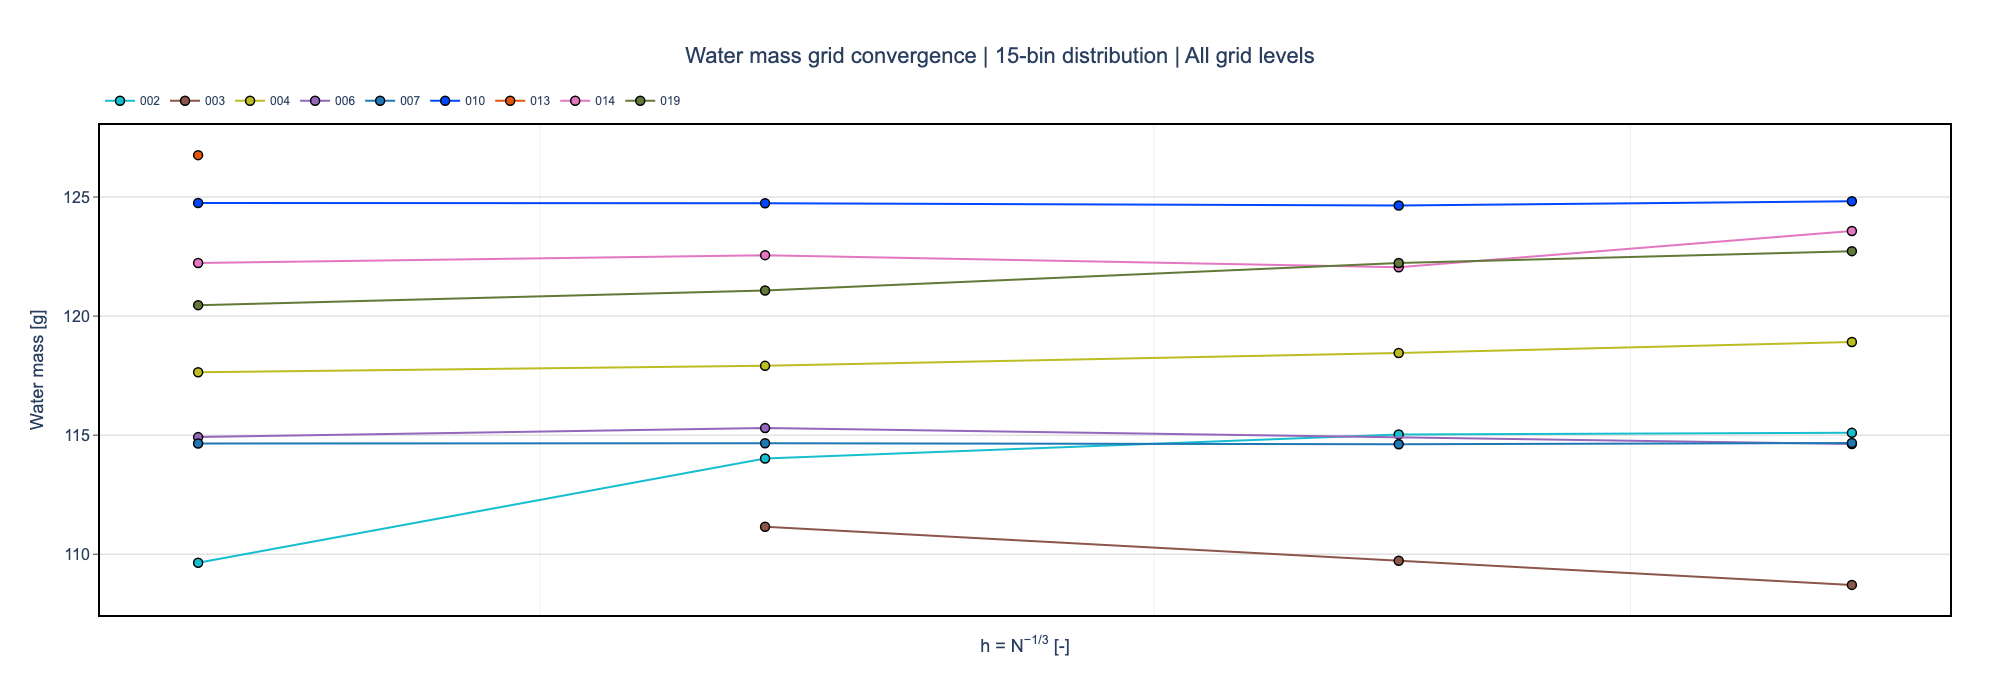
\includegraphics[width=1.0\textwidth]{FIGURES/IMPINGEMENT/tc_naca0012_ae3932_water_mass_vs_n_unspecified_bins15_all_grid_levels.png}
\par}

\vspace{0.15cm}

\begin{block}{\scriptsize Assessment}
\begin{itemize}
    \item For the 15-bin distribution, the L1 median water mass is $119.05~\mathrm{g}$ with an IQR of $6.39~\mathrm{g}$ ($5.37\%$).
    \item Most submissions exhibit weak grid sensitivity, with changes generally within approximately $5\%$ of their L1 prediction.
    \item Code-to-code differences are generally larger than the grid-refinement effect.
\end{itemize}
\end{block}

\end{frame}


% ============================================================
% ============================================================
% NACA0012 -- Droplet Distribution Sensitivity
% ============================================================
% ============================================================

\begin{frame}{\small NACA0012 -- Droplet Distribution Sensitivity}
\scriptsize

{\centering
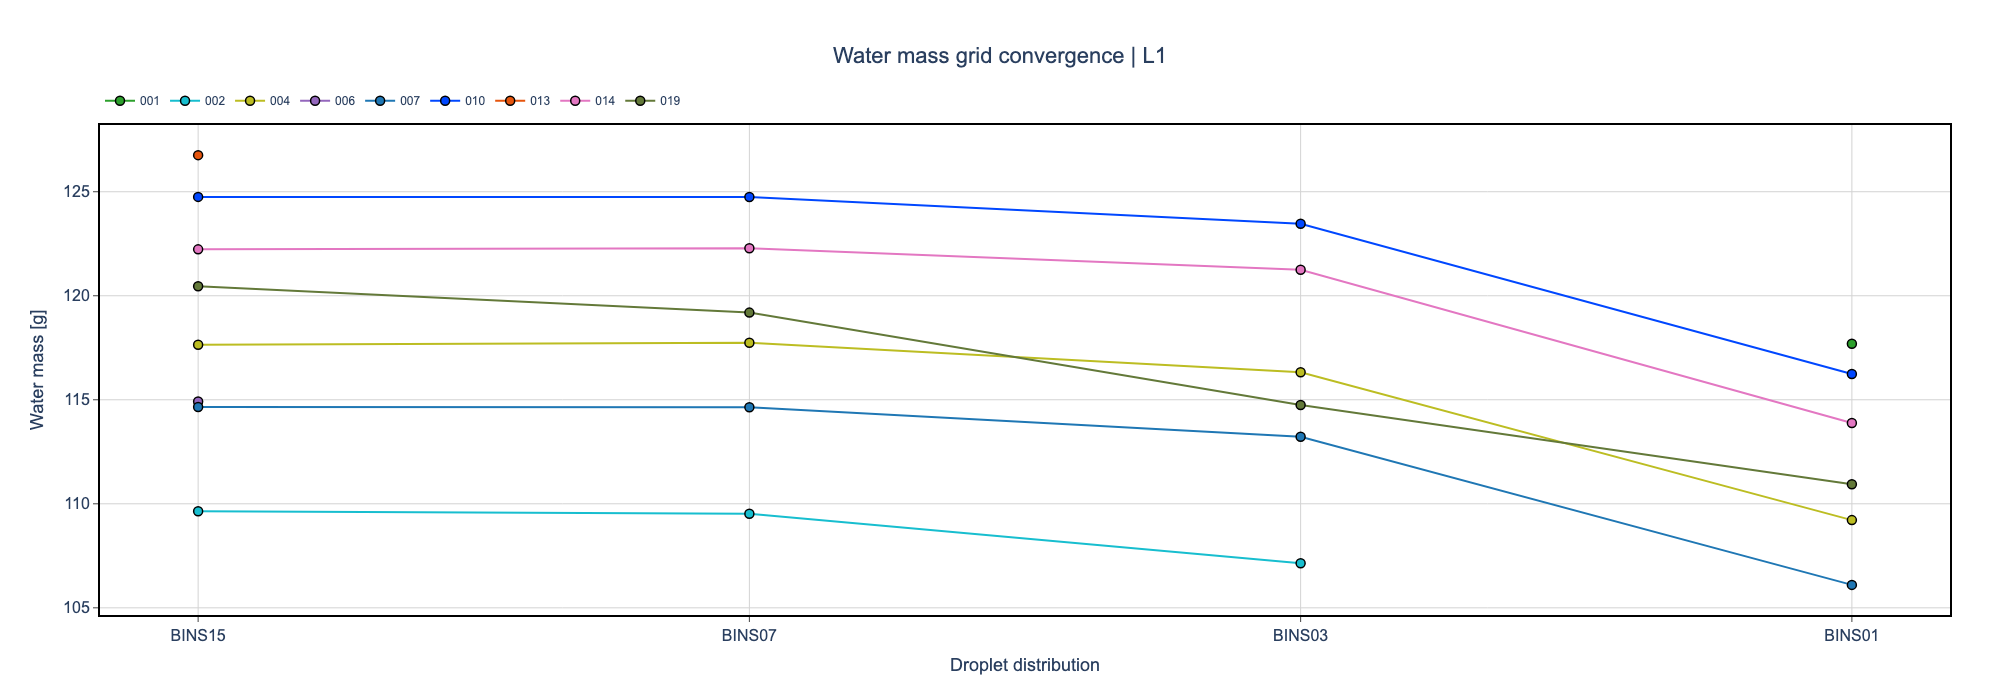
\includegraphics[width=1.0\textwidth]{FIGURES/IMPINGEMENT/tc_naca0012_ae3932_water_mass_vs_n_unspecified_l1_vs_inverse_bins.png}
\par}

\vspace{0.15cm}

\begin{block}{\scriptsize Assessment}
\begin{itemize}
    \item The 15-bin and 7-bin distributions produce very similar impinged water masses.
    \item Reducing the distribution from 7 to 3 bins introduces only a modest change for most submissions.
    \item The single-bin approximation reduces the collected water mass by approximately $5$--$8\%$ relative to the 15-bin distribution for most participants.
\end{itemize}
\end{block}

\end{frame}


% ============================================================
% NACA0012 -- Droplet Impingement Summary
% ============================================================

\begin{frame}[shrink]{\small NACA0012 -- Droplet Impingement Summary}
\scriptsize

\begin{block}{\scriptsize Spatial Grid Convergence}
\begin{itemize}
    \item Weak grid sensitivity is observed for most submissions across both local and integrated impingement quantities.
    \item At L1, the code-to-code spread is $3.0\%$ for $\beta_{\max}$, $2.9\%$ for impingement width, and $5.37\%$ for integrated water mass.
    \item Code-to-code variability generally exceeds the effect of spatial grid refinement.
\end{itemize}
\end{block}

\vspace{0.2cm}

\begin{block}{\scriptsize Droplet-Size Distribution}
\begin{itemize}
    \item The 7- and 15-bin distributions provide very similar integrated water-mass predictions.
    \item The single-bin approximation predicts approximately $5$--$8\%$ less collected water than the 15-bin distribution for most submissions.
    \item Diameter-resolved results show greater scatter for the smallest and largest droplets, while bins near the MVD are more consistent.
\end{itemize}
\end{block}

\vspace{0.2cm}

\begin{block}{\scriptsize Icing-Condition Sensitivity}
\begin{itemize}
    \item Little difference in total water impingement is observed between the two NACA0012 icing conditions.
\end{itemize}
\end{block}

\vspace{0.2cm}

\begin{alertblock}{\scriptsize Takeaway}
Spatial grid refinement has a limited influence on the predicted impingement, whereas droplet-size discretization introduces a more systematic effect. The 7-bin distribution appears sufficient to reproduce the integrated 15-bin result.
\end{alertblock}

\end{frame}


% ============================================================
% ============================================================
% END -- NACA0012 DROPLET IMPINGEMENT
% ============================================================
% ============================================================
